\documentclass{article}
\usepackage{blindtext}
\usepackage{multirow}
\usepackage{amsmath}
\usepackage[utf8]{inputenc}
\usepackage{graphicx}
%bibliography
\usepackage[
    backend=biber,
    style=bwl-FU,
    url=false,
    doi=false,
    eprint=false
]{biblatex}
\addbibresource{Biblio.bib}
\usepackage{threeparttable}
\usepackage{booktabs}
\usepackage{tabularx}
\newcolumntype{L}[1]{>{\raggedright\arraybackslash}p{#1}} % linksbündig mit Breitenangabe
\newcolumntype{C}[1]{>{\centering\arraybackslash}p{#1}} % zentriert mit Breitenangabe
\newcolumntype{R}[1]{>{\raggedleft\arraybackslash}p{#1}} % rechtsbündig mit Breitenangabe
\usepackage{dcolumn}
    \newcolumntype{d}[1]{D{.}{.}{#1}} 

\usepackage[table]{xcolor}
\usepackage[paper=a4paper,left=25.4mm,right=25.4mm,top=25.4mm,bottom=25.4mm]{geometry}

%\usepackage{pgfplotstable}


\begin{document}
\title{Some Visualization}
\author{Tobias Klöpper\thanks{Many thanks especially to Marco, his company and the delicious beer he provides}\\
\normalsize University of Zurich
\and Michele Melek Senkal \thanks{Thanks very much to Marco and each member of this group}\\
\normalsize University of Zürich
\and Marco Barcellos \thanks{Many thanks to all the beers that have allowed me to go on}\\
\normalsize University of Tristan da Cunha
\and David Annoni \thanks{Many thanks to Stack Overflow}\\
\normalsize University of Zurich}
\date{13th of October 2021}
\maketitle
\begin{abstract}
This is Marco practicing some LaTeX Visuals.
\end{abstract}

\newpage
\section{Matlab Plots}
Plots in Figure \ref{fig1} generated with Matlab. I am not sure if color palette is color blind friendly though. I really like the standard Veridian color palette though, even though it's everywhere.

\begin{figure}[!htb]\center 
    \begin{tabular}{cc}
        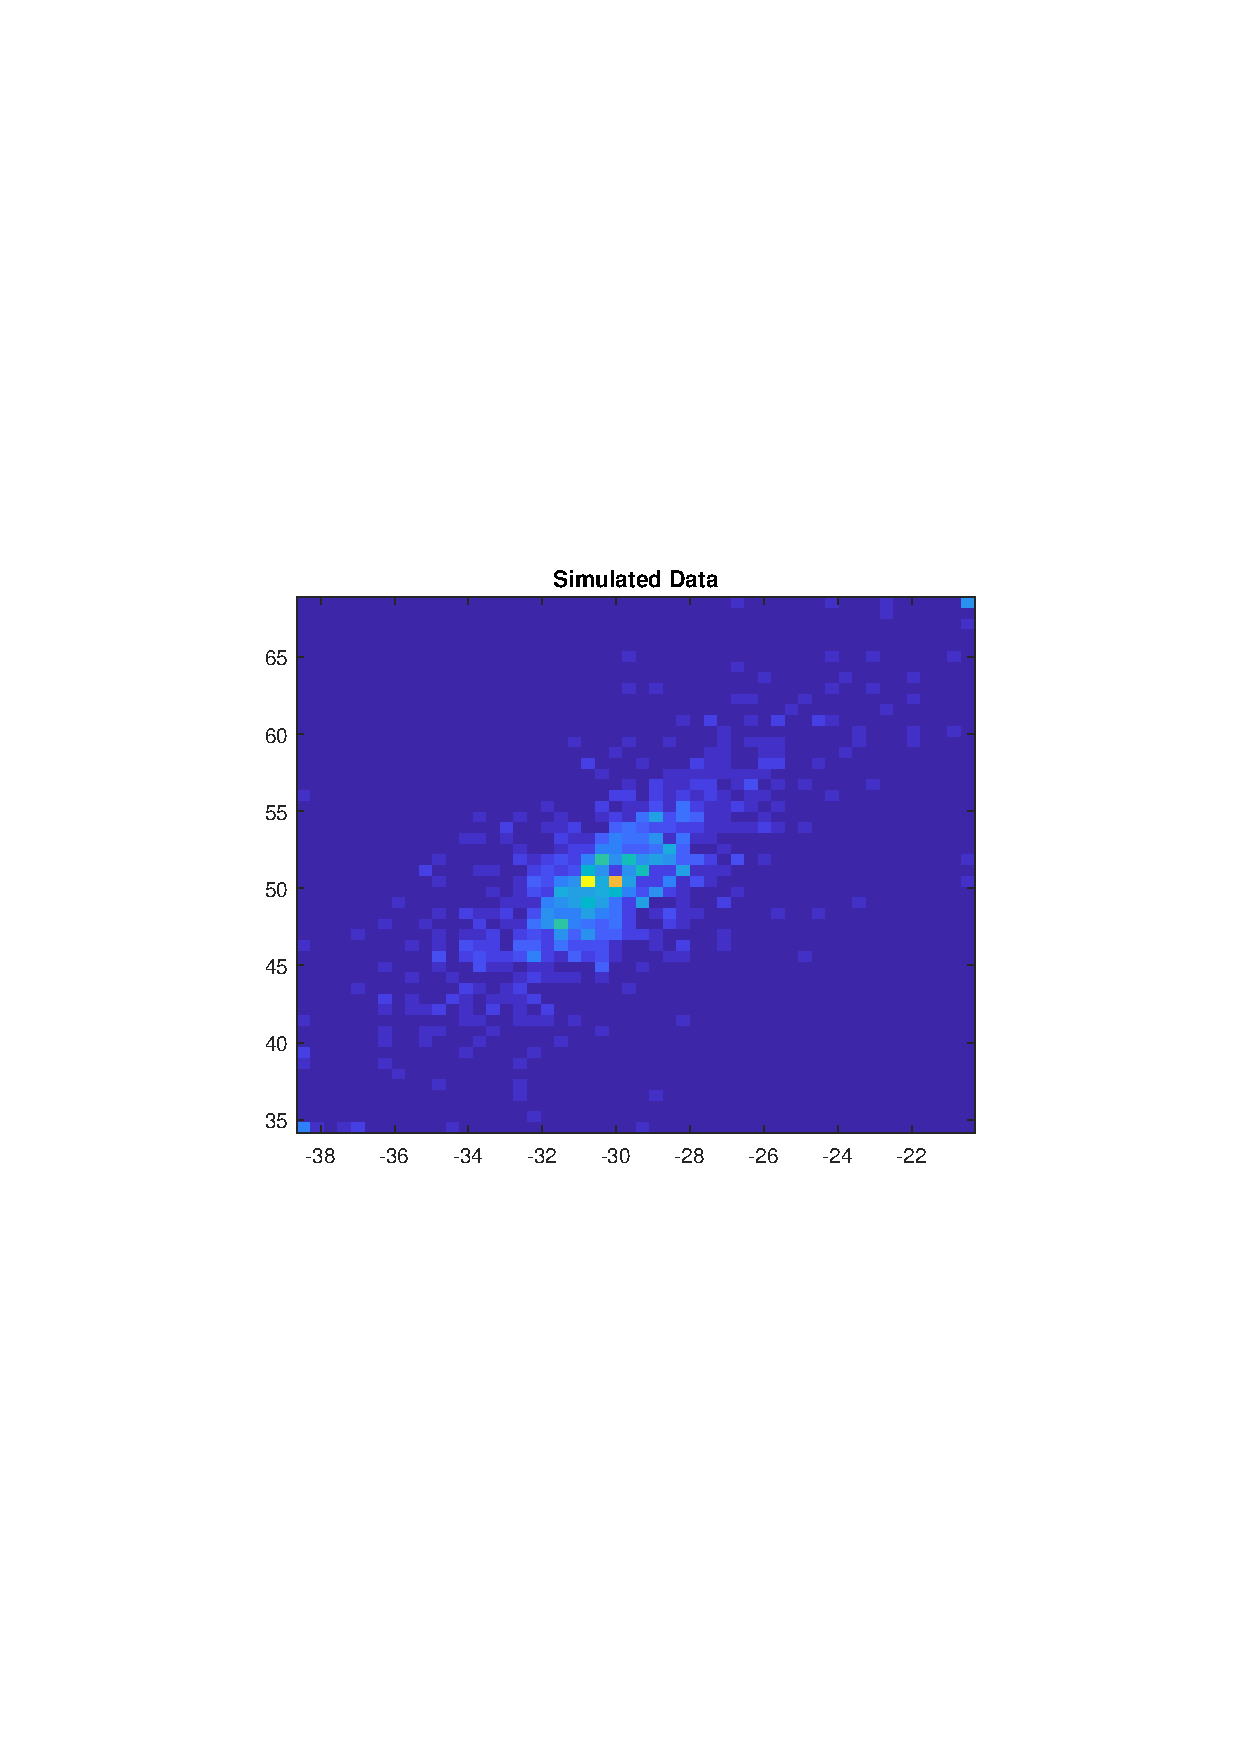
\includegraphics[width=0.5\linewidth, trim = {5cm 10cm 4cm 10cm}, clip]{heat_hist.pdf}
        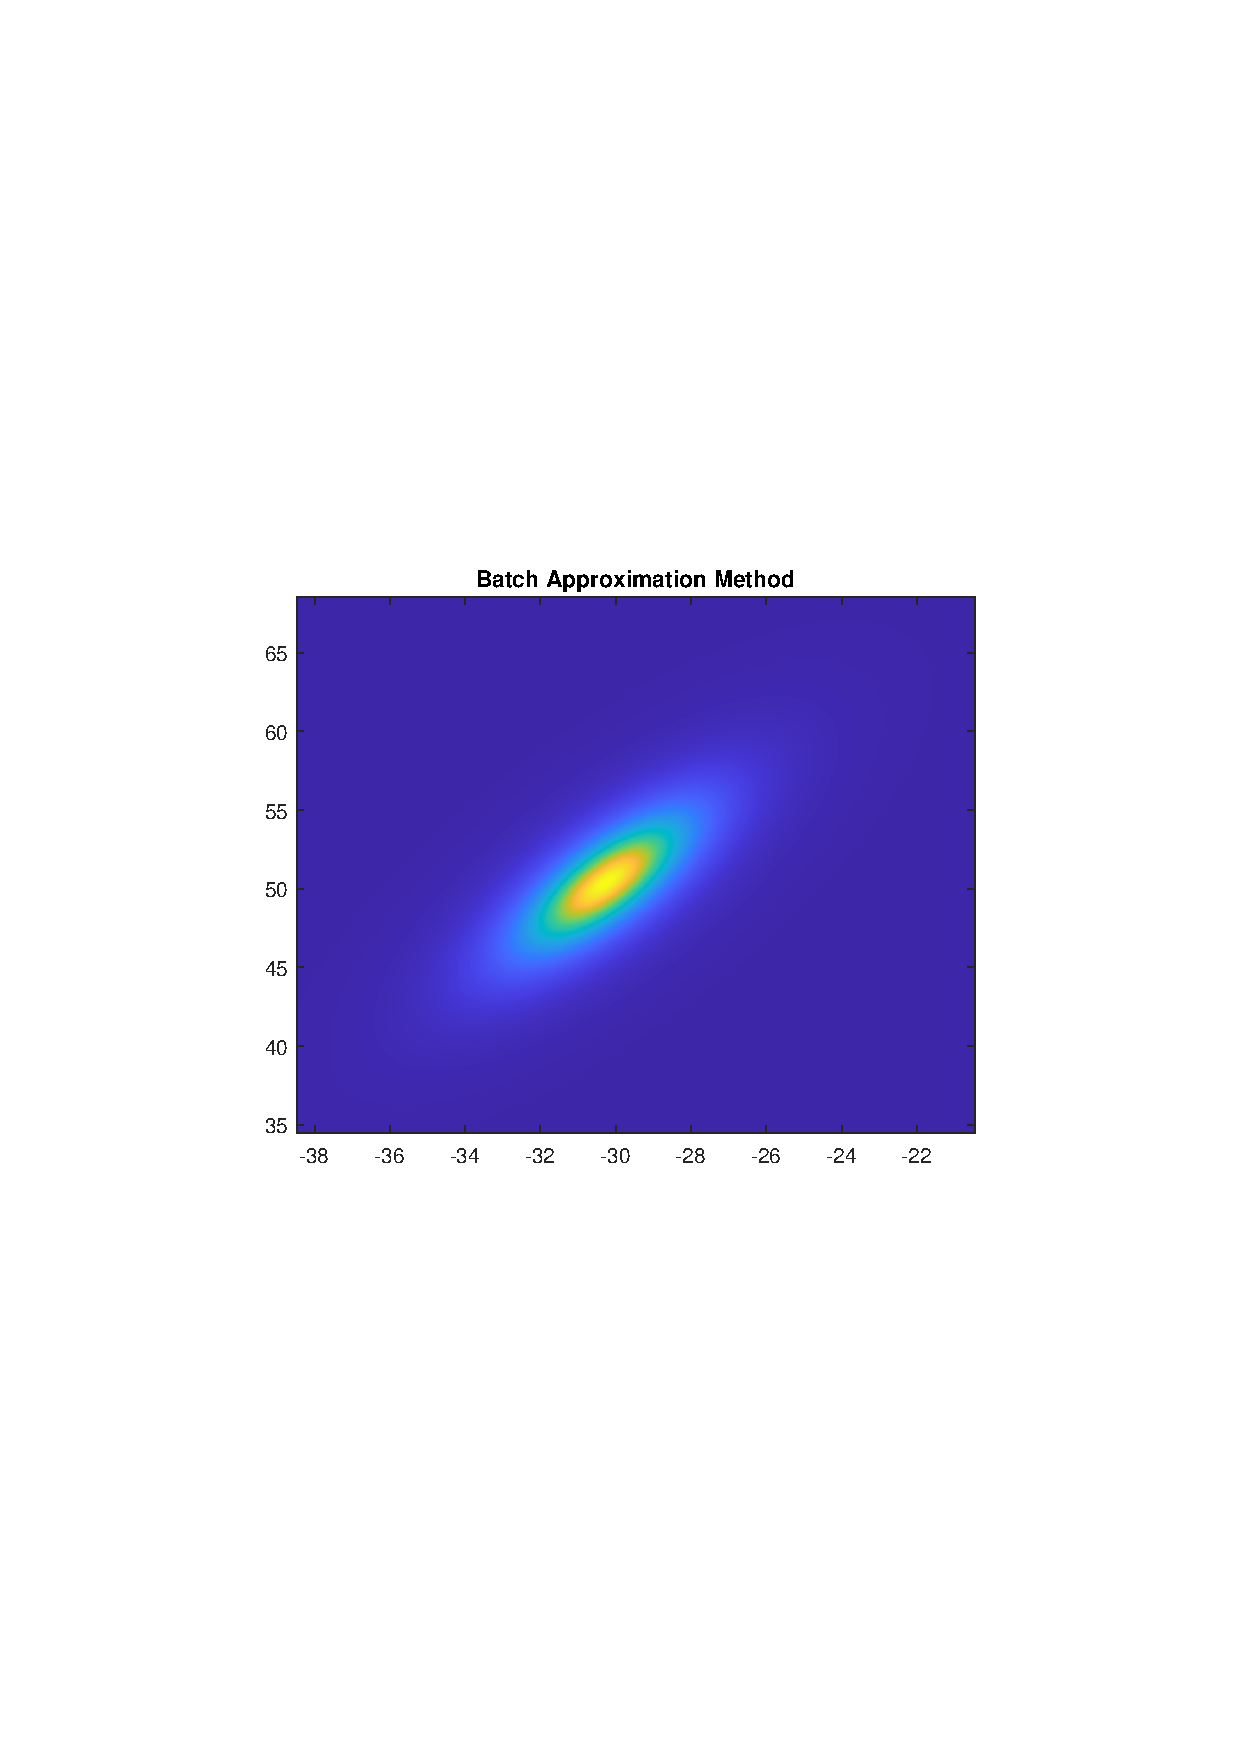
\includegraphics[width=0.5\linewidth,trim = {5cm 10cm 4cm 10cm}, clip]{heat_batch_approx.pdf}
    \end{tabular}
    \caption{\footnotesize Multivariate Student's t Distribution \textbf{Left}: Simulation Heatmap. \textbf{Right}: Batch Approximation Algorithm Estimated Density.}
    \label{fig1}
\end{figure}

\section{R Plots and Table}
\subsection{Plots}
Plots in Figure \ref{fig2} come from R. One of them has a similar color palette as Matlab. The other one I am mostly sure is fine for color blind people.

\begin{figure}[!htb]\center 
    \begin{tabular}{cc}
        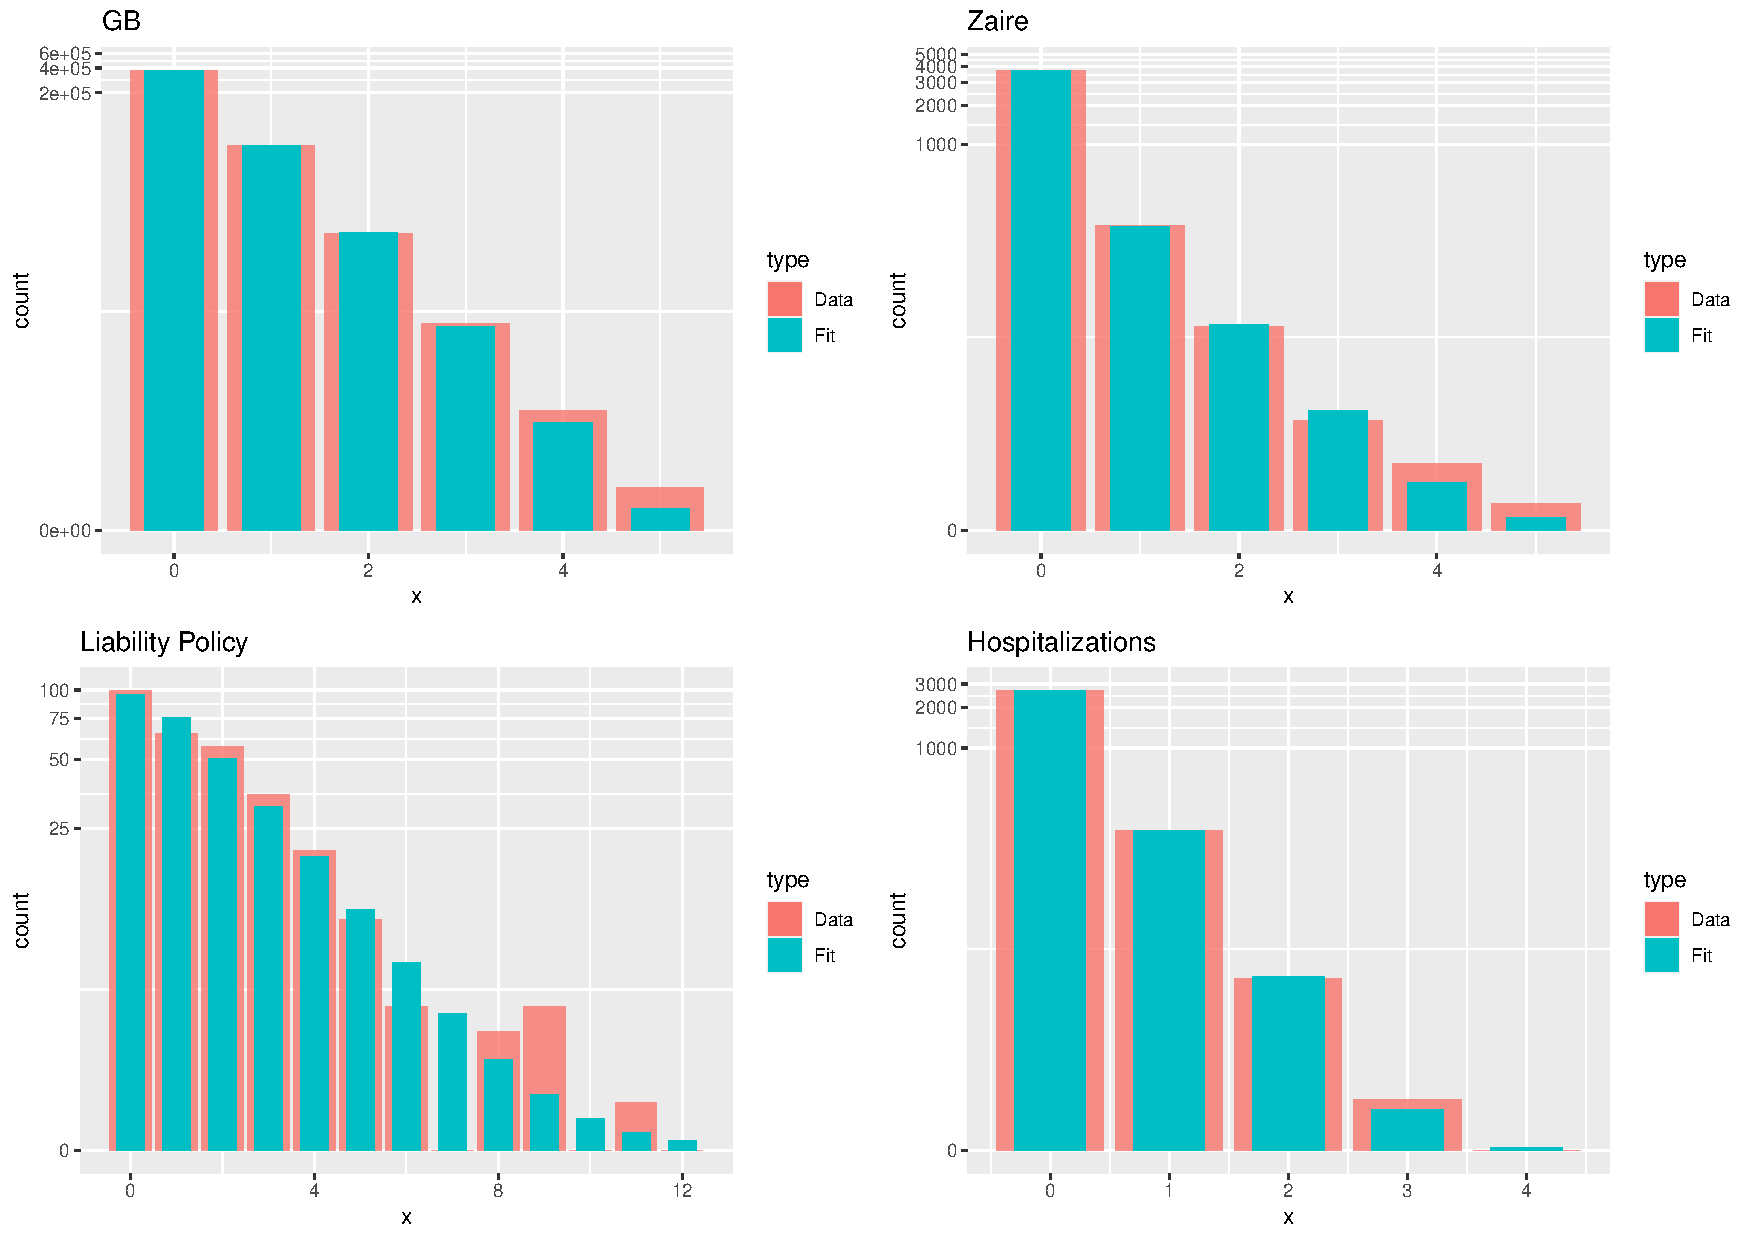
\includegraphics[width=0.5\linewidth, trim = {0cm 0cm 2cm 0cm}, clip]{r_2x2nb.pdf}
        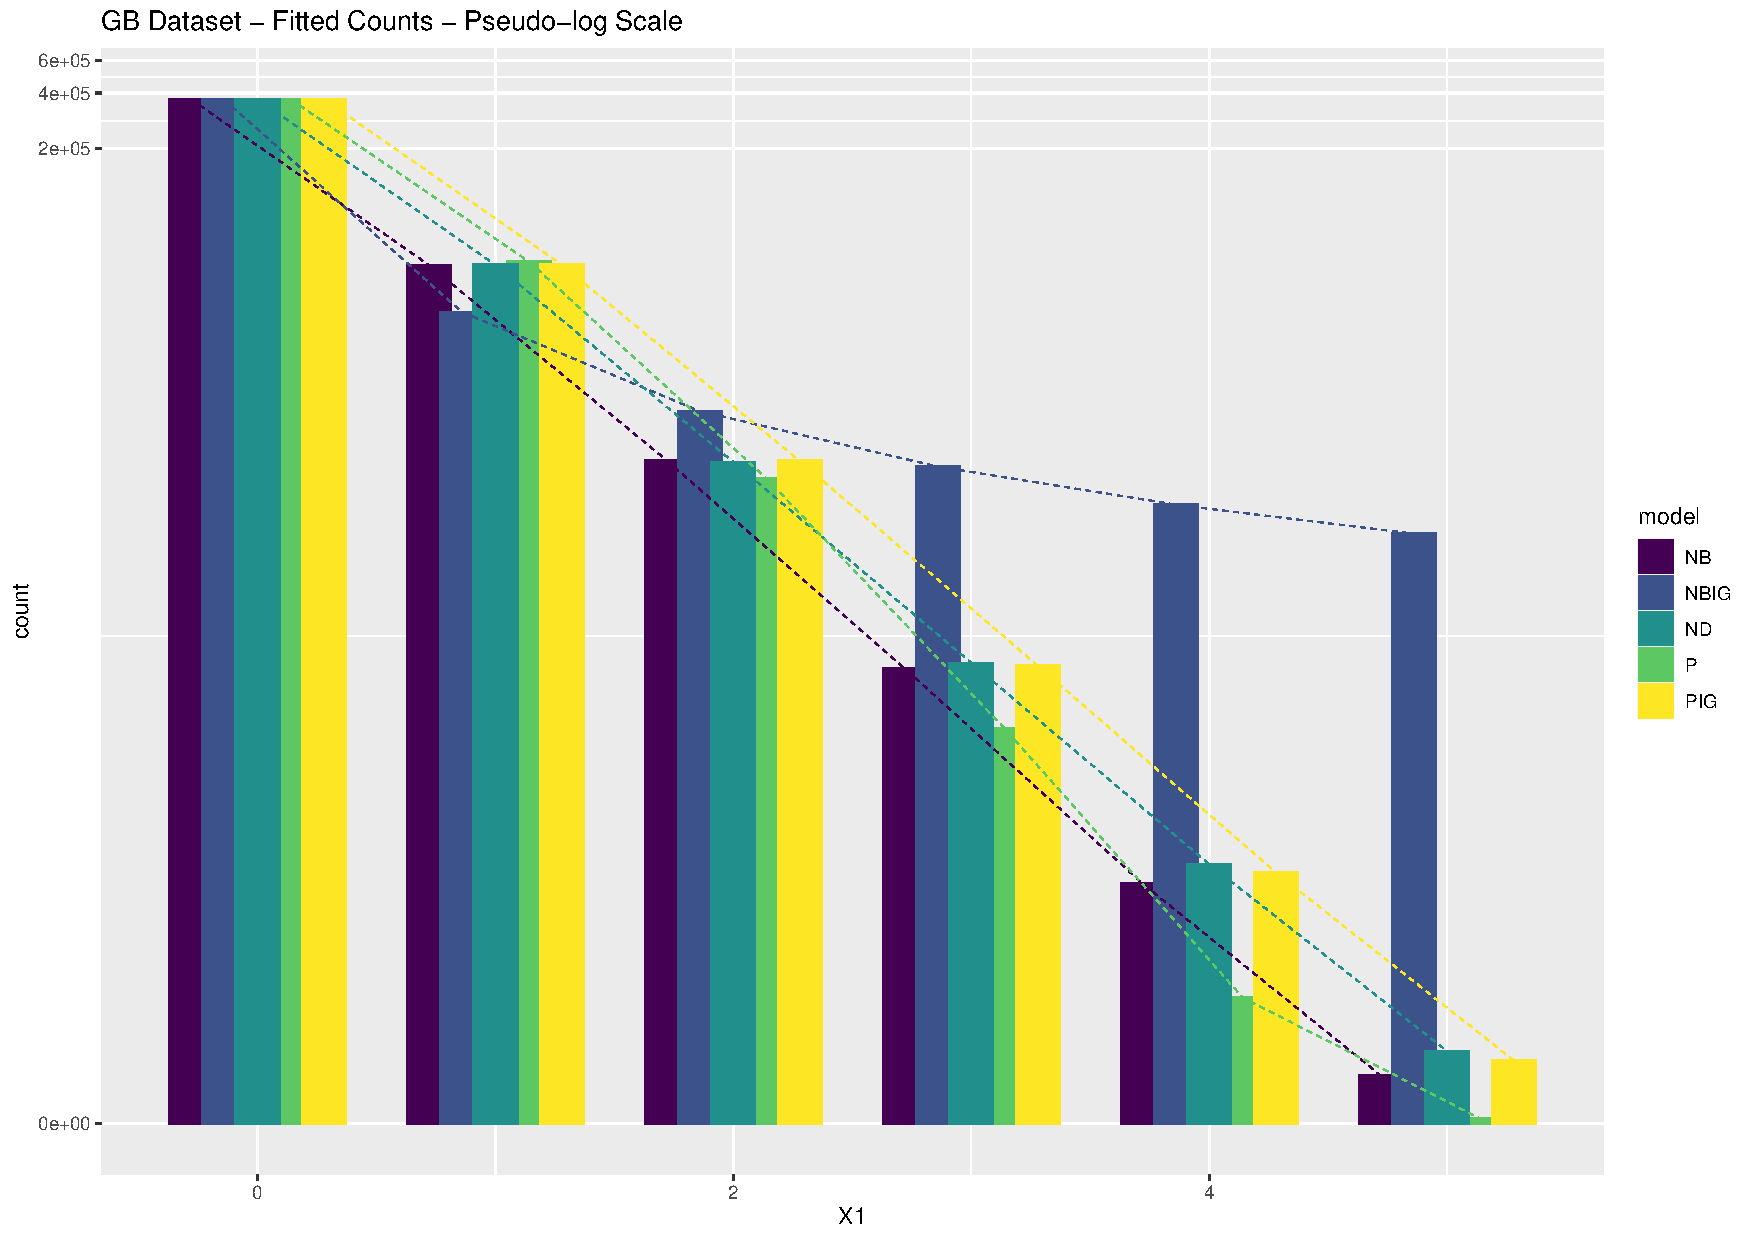
\includegraphics[width=0.5\linewidth,trim = {0cm 0cm 2cm 0cm}, clip]{r_gb_5counts.pdf}
    \end{tabular}
    \caption{\footnotesize Insurance Claim Data from different datasets \textbf{Left}: Data vs. Poisson fit for different datasets. \textbf{Right}: Different fits for a single dataset}
    \label{fig2}
\end{figure}

\newpage
\subsection{Table}
Well, that was really hard.


\begin{table}[h]

  \centering
  \begin{tabular} {l*{7}{d{2}}}

  \toprule
            \multicolumn{7}{|c|}{Fit of automobile claim data in Great Britain, 1968} \\
            \multicolumn{2}{|c|}{}&\multicolumn{5}{|c|}{Fitted values} \\  \midrule  
        No. of claims& Observed & ND & NB & PIG & NBIG & P\\
         0           & 370412 & 370412.91 & 370438.95 & 370435.18 & 369743.74 & 369246.89  \\ 
         1           & 46545  & 46538.25  & 46451.26  & 46476.38  & 25781.37  & 48643.57   \\ 
         2           & 3935   & 3942.39   & 4030.51   & 3995.76   & 7450.47   & 3204.08    \\ 
         3           & 317    & 318.57    & 297.83    & 307.67    & 3726.71   & 140.7      \\ 
         4           & 28     & 25.64     & 20.09     & 23.12     & 2314.76   & 4.63       \\ 
         5           & 3      & 2.06      & 1.28      & 1.75      & 1608.55   & 0.12       \\ 
             \multicolumn{7}{c}{}\\
        Parameter 1 &        &$$\hat{\alpha} = $$ -1.3491   & $$\hat{r} = $$ 2.6047    &$$\hat{\mu} =$$ 0.1317    &$$\hat{\sigma} = $$ 1.516     &$$\hat{\lambda} = $$ 0.1317     \\ 
        Parameter 2 &        &$$ \hat{\theta} = $$ 0.0805    & $$\hat{p} = $$ 0.9519    & $$\hat{\beta} = $$ 0.0512    & $$ \hat{\gamma} = $$ 0.1102    & \\ 
        $\chi^2$&        & 0.67      & 9.13      & 3.24      & 25363.77  & 667.52     \\ 
        $L_{max}$     &        & 171133.3  & 171136.97 & 171134.47 & 195863.3  & 171373.18  \\
  \bottomrule

  \end{tabular}

\caption{Table using dcolumn}     

\end{table}

\section{Heattable}
\def\cca#1{\cellcolor{black!#10}\ifnum #1>5\color{white}\fi{#1}}
\begin{table}[htb]
\label{tab1}
\centering
{\setlength\tabcolsep{1.5pt}%
\begin{tabular}{cccccc}
& $CRO$ & $USA$ & $GER$ & $HUN$ & $POL$ \\
$2020$ &  \cca{0} & \cca{0} & \cca{0} & \cca{2} & \cca{0}\\
$2019$ & \cca{0} & \cca{2} & \cca{0} & \cca{2} & \cca{0}\\
$2018$ & \cca{7} & \cca{4} & \cca{3} & \cca{0} & \cca{4}\\
$2017$ & \cca{3} & \cca{0} & \cca{7} &  \cca{4} & \cca{0}\\
$2016$ & \cca{3} & \cca{7} & \cca{7} & \cca{2} &  \cca{4}\\
$2015$ & \cca{2} & \cca{2} & \cca{7} & \cca{2} & \cca{6}\\
\end{tabular}}
\caption{Average Beer Consumption per day}
\end{table}

\section{Some notes on grids on plots}
Adding grids can be quite helpful when graphs are large and simple ticks along the axis would slow down comprehension. Besides, when barplots are used, grids can be helpful when trying to distinguish their heights when comparing them over large horizontal distances. I do however think that the absence of grids can be quite elegant in some cases, such as when the focus of a plot lies more in displaying a particular feature of a dependency between variables than their magnitudes.
\end{document}